
\documentclass[xcolor={dvipsnames}]{beamer}
\usepackage{amsmath,amsfonts,amssymb,pxfonts,eulervm,xspace}
\usepackage{graphicx}
 \usepackage{multimedia}
\usepackage{media9}
\usepackage{tabularx}
\usepackage{multirow}
\usepackage{minted}

\graphicspath{{./figures/}}
\usetheme{ccnycrest}


\newenvironment{changemargin}[2]{%
\begin{list}{}{%
\setlength{\topsep}{0pt}%
\setlength{\leftmargin}{#1}%
\setlength{\rightmargin}{#2}%
\setlength{\listparindent}{\parindent}%
\setlength{\itemindent}{\parindent}%
\setlength{\parsep}{\parskip}%
}%
\item[]}{\end{list}}

\begin{document}

\title{ CS102: Constants, Math, Formatting}
\author{Hannah Aizenman}

\begin{frame}
	\titlepage
\end{frame}

\begin{frame}[fragile]{Symbolic Constants}
\center
\begin{minted}{c++}
	const double PI = 3.1416;
	const double DEG_TO_RAD = PI/180.0;
	const float AVOGADRO = 6.022e23;
	const int MAXIMUM = 100;
	const string CLASS = "CS102";
\end{minted}

\begin{block}{}
	\begin{itemize}
		\item \textbf{const} means value of var is never changed
		\item used for math/science constants
		\item also used for \textbf{magic numbers}
		\item ALL CAPS by convention
	\end{itemize}
\end{block}
\end{frame}

\begin{frame}[fragile]{Math Library}
	\center
	\huge How do we compute \\the area of a circle? 
	\pause
	\begin{equation*}
	area = \pi r^2
	\end{equation*}
	\pause
	\begin{minted}{c++}
	const double PI = 3.1416;
	double area = PI*r*r;
	\end{minted}
	\pause
	\vspace{.5cm}
	\begin{center} 
	better way to do $r^2$?
	\end{center}
\end{frame}



\begin{frame}{Math Library}
\begin{figure}
	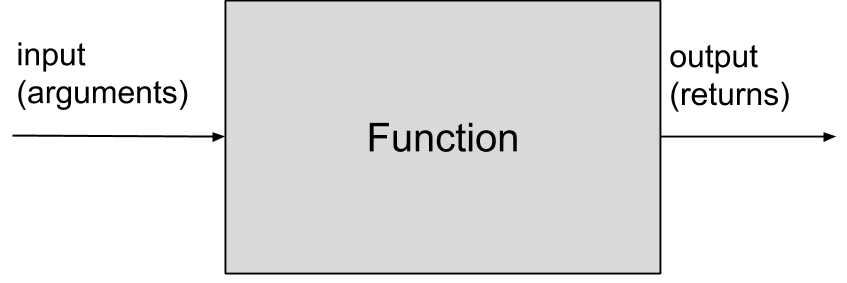
\includegraphics[width=1\textwidth]{function}
\end{figure}
\pause
\begin{block}{Math Equivalent}
\begin{equation*}
	f(x) = y
\end{equation*}
\center
\textbf{x} is the \textbf{input}\\
\textbf{y} is the \textbf{output}
\end{block}
\end{frame}


\begin{frame}[fragile]{Using the Math Library}
\begin{minted}{c++}
#include <iostream>
#include <cmath> //math library

using namespace std;

int main(){
    const double PI = 3.1416;
    int r = 10;
    //pow is in the math library;
    double area = PI*pow(r, 2.0);
    cout<<"Area: "<<area<<endl;
    return 0;
}
\end{minted}
\end{frame} 

\begin{frame}{Common Math Functions}

\begin{tabularx}{\textwidth}{| X | X | X |}
\hline
\textbf{Function Call}& \textbf{Math} & \textbf{Return Type}\\
\hline
\hline
\texttt{abs(a)} & $\lvert x\rvert$ & same type as a\\
\texttt{pow(a,b)} & $a^b$ & same type as a \\
\texttt{sqrt(a)} & $\sqrt{a}$ & \texttt{double}\\
\hline
\hline
\texttt{log(a)} & $\ln(a)$ & \texttt{double}\\
\texttt{log10(a)} & $\log_{10}(a)$ & \texttt{double}\\
\texttt{exp(a)} & $e^{a}$ & \texttt{double}\\
\hline
\hline
\texttt{sin(a)} & $\sin(a)$ & \texttt{double}\\
\texttt{cos(a)} & $\cos(a)$ & \texttt{double}\\
\texttt{tan(a)} & $\tan(a)$ & \texttt{double}\\
\hline
\end{tabularx}
\end{frame}

\begin{frame}[fragile]{Better Output}
\begin{minted}{c++}
#include <iomanip>//library for formatting output
//...code
cout<<"Area: "<<setiosflags(ios::fixed)
    <<setprecision(3)<<area<<endl;
//...more code
\end{minted}

\begin{block}{}
	\begin{itemize}
		\item \texttt{cout} can span multiple lines
		\item formatters need to come before what they're formatting
		\item formatters can be changed
		\item these formatters modify how area is outputted
		\item \texttt{endl} means print a newline
	\end{itemize}
\end{block}
\end{frame}

\begin{frame}{Format Functions}
\begin{tabular}{|l|l|}
\hline
\textbf{Manipulator} & \textbf{What it Does} \\
\hline
\texttt{setw(n)} & set the field width to \texttt n \\
\hline
\texttt{setprecision(n)} & set the floating point precision \\
			    & fixed flag is set:\\
			    & \texttt{n} is the number of decimals \\
			   & otherwise: \\
			   & \texttt{n} is the number of significant figures\\
\hline
\texttt{setfill(C)} & set the leading fill character to \texttt{C}\\
  		    	& a space character is the default fill\\
\hline
\texttt{setiosflags(flags)}    & set the format flag to true\\
				& format flags control output\\
\hline
\end{tabular}
\end{frame}
\begin{frame}{Format Flags}
\begin{tabular}{ | l|l|}
\hline
\textbf{Flag} & \textbf{Meaning} \\
\hline
\hline
\texttt{ios::fixed} & always show decimal (6 places by default)\\
		       & even if the number is large\\
		       & pad with zeros if necessary\\
\hline
\texttt{ios::showpoint}&  same as \texttt ios::fixed\\
			    & reverts to exponential for large numbers\\
			    &\texttt ios::fixed takes precedence\\

\hline
\hline
\texttt{ios::scientific} & output in exponential format\\
\hline
\texttt{ios::showpos} & display a + before positive numbers \\
\hline
\texttt{ios::boolalpha} & output booleans as true/false\\
\hline
\hline
\texttt{ios::left} & left or right justify output\\
\texttt{ios::right} &\\
\hline
\hline
\texttt{ios::dec} &display  numbers in dec, hex, or octal\\
\texttt{ios::hex} & \\
\texttt{ios::oct} & \\
\hline
\texttt{ios::showbase} & display which base the number is in\\
\hline
\end{tabular}
\end{frame}

\end{document}